%---------------------------------------------------------------------------------------
\chapter{Ideia}

A fim de implementar um sistema que trate dos problemas citados e consiga atingir os objetivos propostos, são necessários processos e a utilização de determinadas tecnologias, citadas no subtópico . 

Os processos principais são três, o cadastramento dos usuários, a automatização do \ac{fpa} e a possibilidade de habilitação de outros processos, por parte dos administradores, com destaque à permutação dos horários já atribuídos e à desativação de um docente em determinada matéria.

\section{Cadastramento dos usuários}

Preliminar à qualquer utilização do \ac{ada}, o Administrador Superior (\gls{superAdmin}), será cadastrado pelos próprios programadores e terá o maior nível de acesso, podendo realizar quaisquer alterações e controlar quais serão os Administradores (\gls{admin}). 

Então, os outros funcionários receberão um link para acessarem o \ac{ada} via Google, pelo e-mail institucional - o que evita acessos não permitidos, e serão atribuídos instantaneamente ao papel de Professor (\gls{professor}); como mencionado, a mudança desse nível de acesso para o de \gls{admin} é realizada pelo \gls{superAdmin}. E acessos posteriores poderão ser através do Google ou do prontuário e senha.

\subsection{Configuração do ambiente}

A configuração do ambiente é um subprocesso, em que o \gls{superAdmin} será responsável por habilitar a possibilidade de \glspl{permuta} e de desativação do docente em uma disciplina; prazos limites à organização; e definição ou atualização dos critérios da atribuição - baseados na legislação vigente e na ordem de prioridade de escolha das disciplinas.

E o \gls{admin} será responsável pela subárea, consequentemente, por subir a grade horária; determinar prazos específicos; autorizar a \gls{permutação} e se deseja participar da aprovação das \glspl{permuta}; controlar os docentes desativados; e adicionar\footnote{Essa adição será manual e de acordo com a prioridade escolhida. Portanto, um subprocesso, onde o \gls{admin} colocará os docentes na ordem e, igualmente, poderá alterá-la em caso de erro ou modificações futuras.} os que participarão de sua subárea. 


\begin{figure}[h]
    \centering
    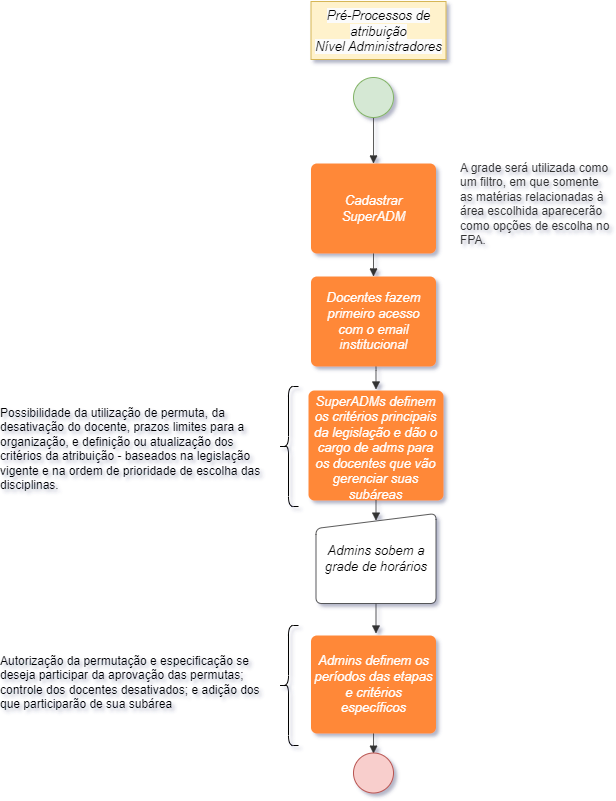
\includegraphics[width=0.85\textwidth]{anexos/Fluxograma/FluxogramaCadastramento.png}
    \caption{Fluxograma dos pré-processos de atribuição}
    \label{fig:figura1} 
\end{figure}

\section{Automatização do FPA}

Finalizada a organização do sistema pelos administradores e todos os docentes cadastrados nas subáreas, eles poderão acessar o sistema e iniciar o processo de escolha da disponibilidade de horários e da preferência de aulas (prioritária e secundária) e de atividades. Conforme é realizado esse processo, o ADA verifica se cada escolha segue os regramentos, e impossibilita a escolha de disciplinas em conflito; igualmente, informa com uma mensagem breve caso o docente selecione uma em que foi desativado. 

\begin{figure}[t]
    \centering
    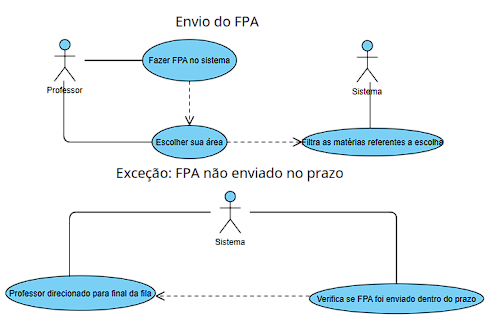
\includegraphics[width=0.7\textwidth]{anexos/CasosDeUso/CasoDeUso_EnvioFPA.png}
    \caption{Caso de uso do envio de preferências}
    \label{fig:figura2} 
\end{figure}

A determinação da preferência de atividades poderá ser modificada dentro do prazo de entrega estabelecido pelo \gls{admin}. Porém, ao encerrar o prazo, o \ac{ada} percorre a lista de docentes, em ordem decrescente, e atribui as aulas de acordo com o selecionado. O processo é interrompido - e é armazenado o que já foi feito - caso haja conflito com uma disciplina já escolhida; assim, aquele docente receberá uma solicitação para alterar sua escolha dentro de determinado prazo.

\begin{figure}[h]
    \centering
    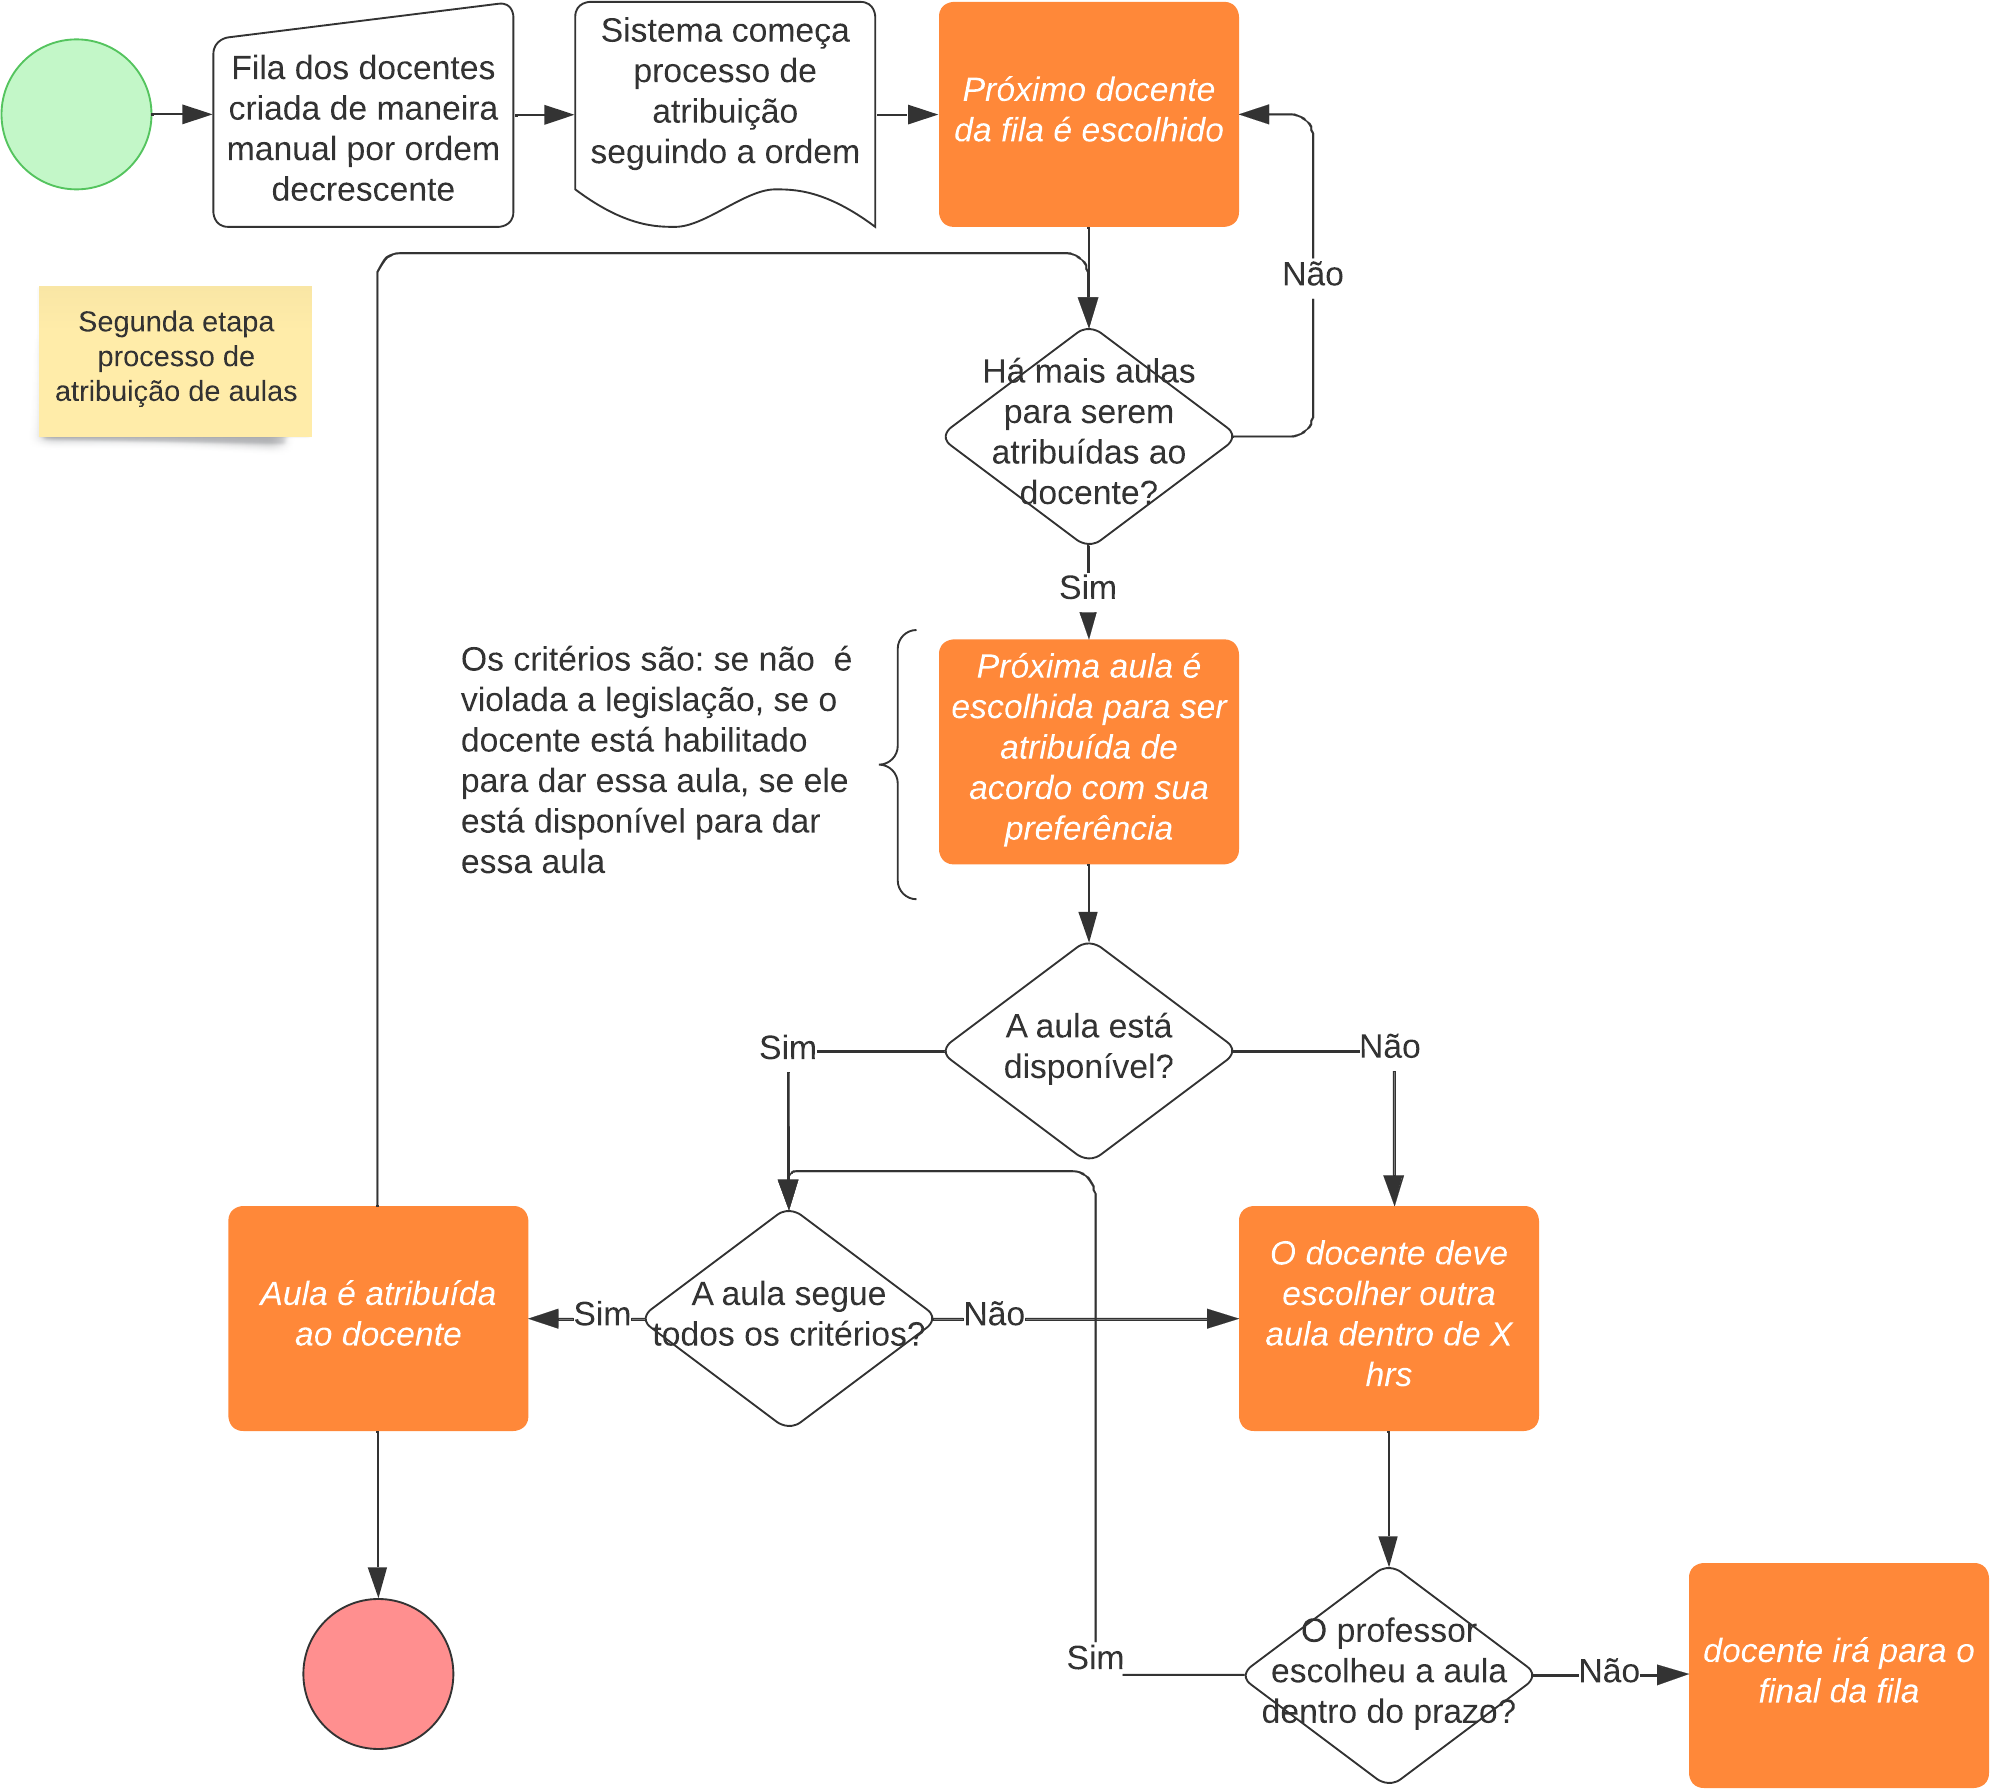
\includegraphics[width=0.7\textwidth]{anexos/Fluxograma/FluxogramaProcessoAtribuicaoAulas.png}
    \caption{Fluxograma da atribuição de aulas}
    \label{fig:figura3}
\end{figure}

\section{Permutação}

A permutação é aberta, caso habilitada com a conclusão da grade pelo sistema. De modo geral, é feita com a solicitação de um docente pela troca de sua aula por uma específica do outro, selecionada na grade. É impossibilitada mais de uma solicitação, ao mesmo tempo, para uma mesma aula; Apenas é liberada quando essa for aceita ou recusada. Igualmente é impossibilidada a solicitação de alguma que descumpra o regramento. 
Caso o \gls{admin} seja moderador, ele terá que aprovar a aceitação da permuta pelo segundo docente.


Por fim, é gerada a grade horária final, onde os docentes e os administradores conseguem visualizar e salvar a atribuição de aulas da subárea. Além da possibilidade de gerar o \ac{fpa} com essa grade pronta.

\begin{figure}[h]
    \centering
    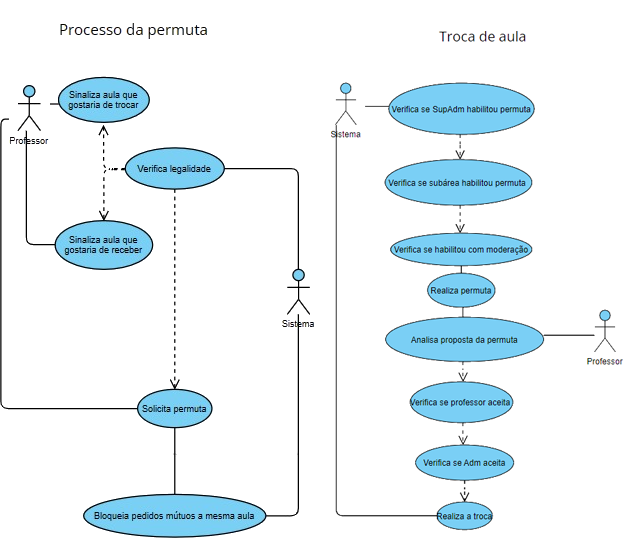
\includegraphics[width=1\textwidth]{anexos/CasosDeUso/CasoDeUso_ProcessoPermutaFULL.png}
    \caption{Caso de uso troca de Aula}
    \label{fig:figura4} 
\end{figure}

\section{Tecnologias e ferramentas aplicadas}

Em vista do desenvolvimento do \ac{ada} de maneira concisa e eficaz, a implementação de tecnologias e suas respectivas ferramentas se faz necessária. Além disso, repositórios de controle de versão e Integrated Development Environment (\ac{ide}) deverão, e serão, utilizadas.

\subsection{Desenvolvimento do sistema}
 É baseado nas metodologias ensinadas no projeto \gls{codelab}, para manter uma padronização e pela maior afinidade dos integrantes com as linguagens e os \textit{\gls{framework}}. No \gls{backend}, será utilizado o \gls{springboot}, um \textit{\gls{framework}} \textit{open source} da linguagem Java. E, no \gls{frontend}, o \textit{\gls{framework}} \textit{open source} \gls{angular}, com base na linguagem \gls{typescript}, e detalhes específicos em \ac{css3}. Para o gerenciamento de dados, o Sistema de Gerenciamento de Banco de Dados (\ac{sgbd}), pelo \gls{mysql}.  
 
Ademais, à vista de promover uma aplicação segura, o sistema seguirá uma sequência de métodos que aplicam o formato \gls{https}, e utilizará o \gls{jwt}, um padrão da Internet que visa a autenticação dos usuários no sistema.

\subsection{Controle de Versão e Implementação}
Terá a utilização do Subversion/Subversão (\gls{svn}) como repositório principal, e do \gls{github} como repositório secundário, devido ao melhor gerenciamento de branchs e o armazenamento em outro local de informações, em caso de algum erro no \gls{svn}. Ele será atualizado quinzenalmente com o conteúdo do principal. 
E o código será implementado em um editor de código-fonte, o \ac{vscode} - desenvolvido pela \gls{microsoft}.


%---------------------------------------------------------------------------------------





